\chapter{Evaluation}\label{chap:ContCaptions}
To show the effectiveness of ColStream, Zhong et al. provide in \cite{ColStream} measurements they have collected in experiments. The scenarios for these experiments focus on its features, and one is a comparison with the COMBINE tool. The first is the increase of throughput by means of utilizing the network connection of several devices. The second is the adaptation to a changing number of available collaborators. We discuss these measurements in the following chapter. In the following four sections we discuss the experiments and results presented in \cite{ColStream} and point out aspects we consider problematic. The names of the respective sections follow the titles used in the paper.
\section{Experiment A: "basic tests"}
\subsection{Measurement Setup}
In these experiments ColStream runs on emulated android devices. One initiator and up to ten collaborators are emulated on a computer with an Intel Core i5-3210M processor and 6 GB of RAM. The paper claims that the throughput available to the individual emulated devices was fluctuated to make their behaviour more realistic, however the exact process of fluctuation is not disclosed. The initiators stream one of three videos from Youtube. These videos were randomly selected and differ in size. The time it takes for them to download the video was measured. The measurements were repeated with varying number of collaborators. 
\subsection{Results}
\begin{figure}[hbt]
\centering
\caption{Performance over number of collaborators \cite{ColStream}}
\label{performanceResults}
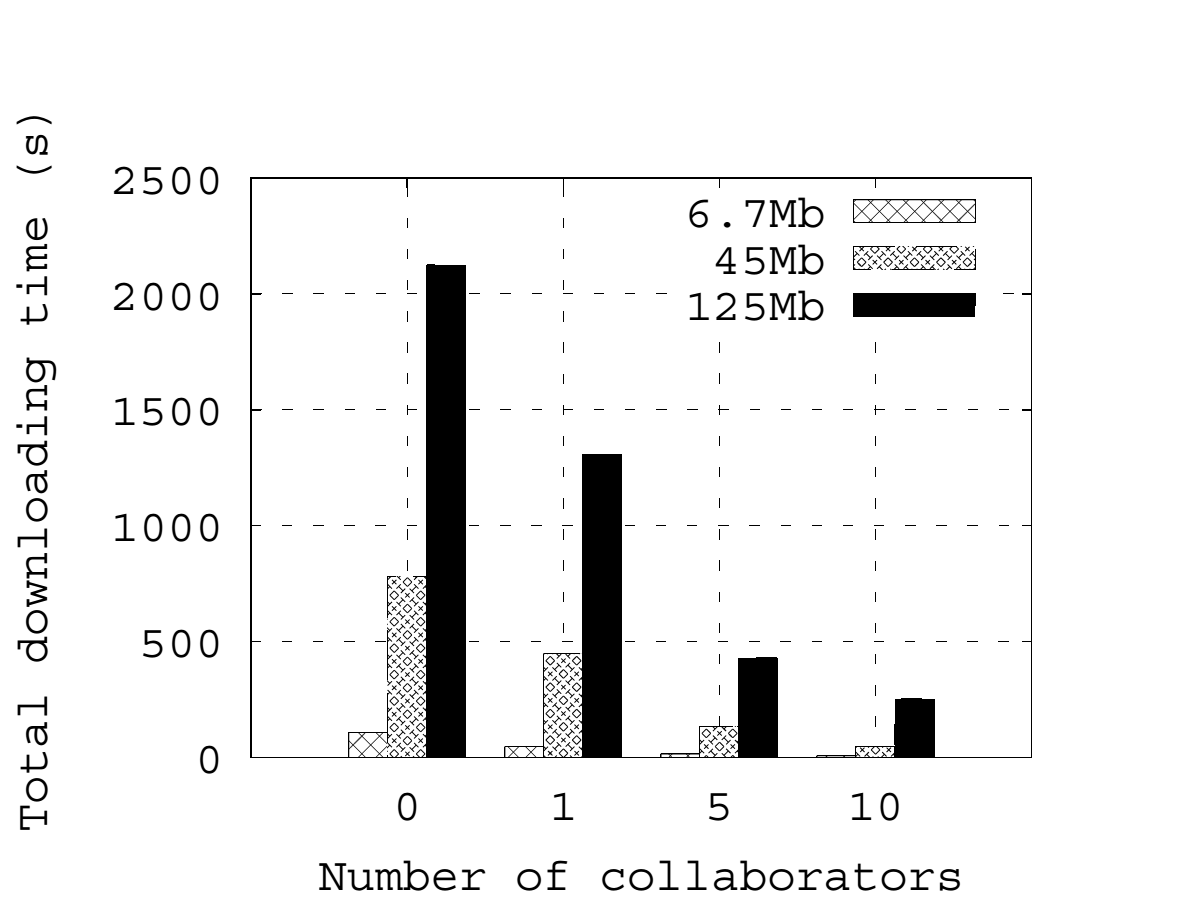
\includegraphics[scale=.5]{figures/Results.png}
\end{figure}
Figure \ref{performanceResults} shows the results as measured by Zhong et al. as a bar graph. The values are grouped by the number of collaborators used. Within each group, the time it took for this configuration to download each of the three videos is shown in seconds by the height of the corresponding bar. The size of the corresponding video for the bar is indicated by the pattern applied to it. This experiment shows that ColStream is able to reduce the time it takes to stream a video through employment of additional collaborators. In all three filesizes, the use of one collaborator already reduces the time by about a third. The improvement appears to increase with the size of the video to download.

\subsection{Criticism}
There are several aspects that raise the question if these results can be applied to a real world scenario. The paper provides very little information on the simulated network available to the emulated devices. One of the key motivations for the creation of ColStream is the compensation for fluctuation of throughput. Without knowing the strentgh of fluctuation applied to the throughput available to the streaming devices, these measurements can not be properly evaluated. Additionally these fluctuations seem to have been applied on the simulated 3G/LTE connection only, not on the Wi-Fi connection between the individual devices. The measurements were not repeated with different streaming platforms, files, networks or in any other variation. While these measurements do show as intended that ColStream could work, they do not show that it will work in any reliable way.


\section{Experiment B: "Dynamic adaptation"}
This experiment intends to show that ColStream is able to react to a changing group of collaborator. To do so, the streaming behaviour in reaction to collaborators joining and leaving the groups as well as price changes are demonstrated.
\subsection{Measurement Setup}
Unfortunately the measurement setup for this experiment is not explicitly stated. We assume the basic setup to be the same as in Experiment A, with emulated devices running on a notebook and experiencing a simulated fluctuation of network throughput. Three different situations are simulated. Number one is a new collaborator joining the group and demanding a lower price then the previously available collaborators. Number Two is a collaborator leaving the group. Number three is the loss of connection to one of collaborators.
\subsection{Results}
\begin{figure}[hbt]
\centering
\caption{Download ammunt over time by collaborator with user joining \cite{ColStream}}
\label{ColStreamJoin}
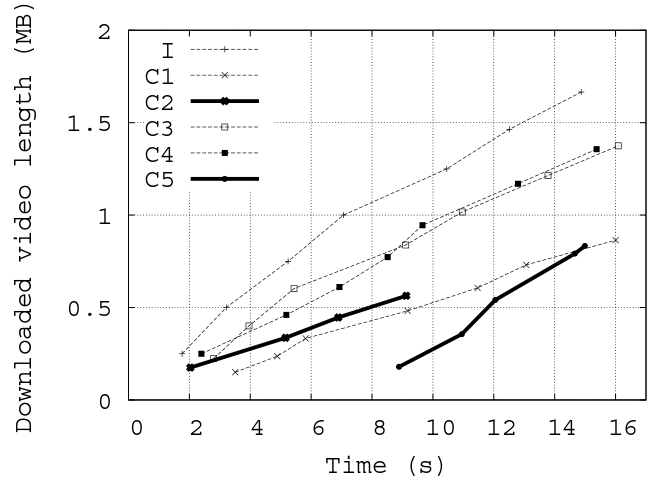
\includegraphics[scale=.5]{figures/ColStreamJoin.png}
\end{figure}
\begin{figure}[hbt]
\centering
\caption{Download amount over time by collaborator with user leaving \cite{ColStream}}
\label{ColStreamLeave}
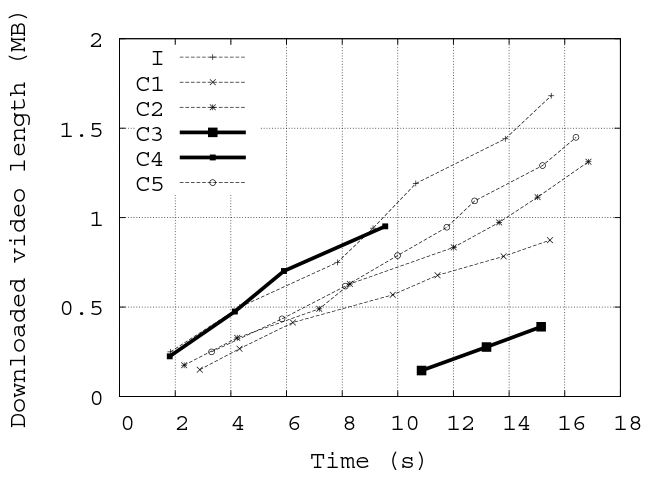
\includegraphics[scale=.5]{figures/ColStreamleave.png}
\end{figure}
\begin{figure}[hbt]
\centering
\caption{Download amount over time by collaborator with connection loss to user \cite{ColStream}}
\label{ColStreamReJoin}
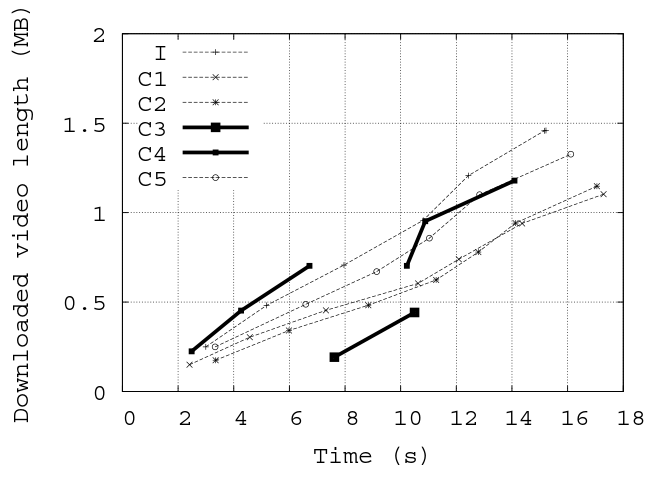
\includegraphics[scale=.5]{figures/ColStreamReJoin.png}
\end{figure}
The figures \ref{ColStreamJoin}, \ref{ColStreamLeave} and \ref{ColStreamReJoin} show the accumulated downloaded amount of data by collaborator over time. In all three figures the collaborators behave as expected. In figure \ref{ColStreamJoin} we see a new user (C5), demanding a lower price join after 9 seconds. As a result the user C2 is no longer assigned new parts to download. In figure \ref{ColStreamLeave} we see a user (C4) orderly leave and another user (C3) being selected as his replacement. Figure \ref{ColStreamReJoin} shows that colstream is able to handle a connection loss (at around 7 seconds) and its reestablishment (shortly after 10 seconds) to a collaborator(C4).
\subsection{Criticism}
While these measurements do suggest that ColStream could work as promised, unfortunately the influence of the collaborators leaving and joining on the quality of a videostream for the user is not made clear.

\section{Experiment C: "Performance tests: COMBINE agains ColStream"}
This experiment compares ColStream and COMBINE, which is also discussed in Section \ref{relWork} and intends to show that ColStream is better prepared to handle the specific challenges of distributed video streaming. To compensate for possible packet loss, chunks are assigned to multiple collaborators, to be sure to receive the information in time. This experiment looks at the amount of data that needs to be redownloaded by both systems, in reaction to random failures of collaborators.
\subsection{Measurement Setup}
Again very little is said to the setup of the experiment besides the use of five collaborators. While we can assume ColStream to be set up in a similar way as in the previous experiments, no such assumptions can be made about COMBINE.
\subsection{Results}
\begin{figure}[hbt]
\centering
\caption{Redownload handling by ColStream and COMBINE \cite{ColStream}}
\label{ColStreamCOMBINEComparisom}
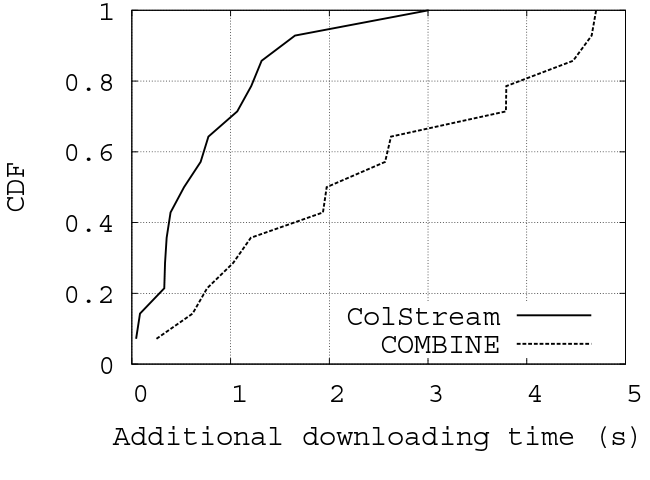
\includegraphics[scale=.5]{figures/ColStreamCOMBINE.png}
\end{figure}

Figure \ref{ColStreamCOMBINEComparisom} shows the performance of ColStream and COMBINE with growing additional downloading time on the x axis and their scores in a not exactly defined cumulative distribution function based benchmark on the y axis. ColStream is scoring higher at all measured values.
\subsection{Criticism}
Unfortunately it is in no way clear how reliable these benchmark tests are.

\section{Experiment D: "Feasibility study of the optimisation algorithm"}
This experiment measures the time it takes for ColStream to adjust to changing collaborator groups. This measurement allows to evaluate the amount of overhead generated by the group management and to decide if an initiator can adjust his peer selection fast enough to properly leverage changes in the group.
\subsection{Measurement Setup}
This experiment was executed on real devices with a range of hardware capabilities, specifically an HTC Desire C, Samsung Galaxy Nexus and a Samsung Note II. It was repeated for varying group sizes ranging from one to fifty participants. The time it took the initiator to adjust its peer selection is measured. Unfortunately it is not made clear if a video was streamed during this experiment.
\begin{figure}[hbt]
\centering
\caption{Group optimisation over group size \cite{ColStream}}
\label{groupAdjustment}
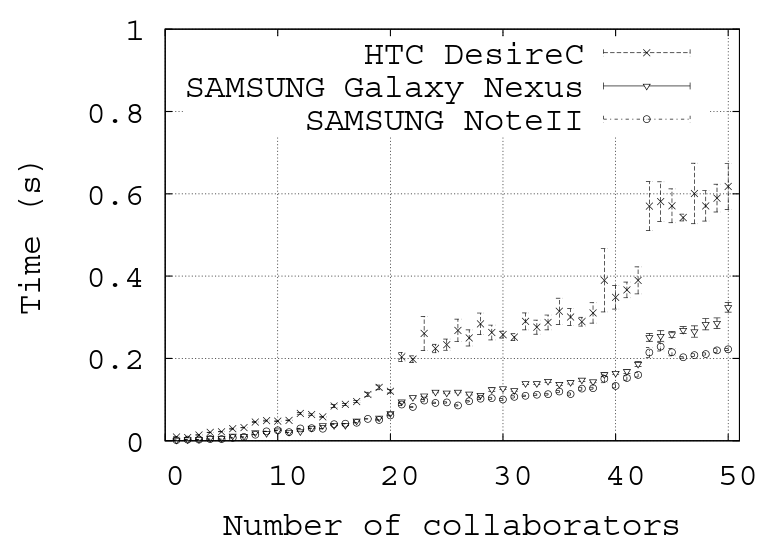
\includegraphics[scale=.5]{figures/ColStreamAdjustment.png}
\end{figure}
\subsection{Results}
Figure \ref{groupAdjustment} shows the group adjustment time on the y axis over group size on the x axis for the three devices. A clear trend of the adjustment time growing with the group size is visible. While the values for the two Samsung devices are close together, the Desire C takes longer to adjust.
This fits the much lower hardware characteristecs of the HTC device compared to the Galaxy Nexus. The Note II is the only device with a multi core processor. Since the peer selection algorithm is in no way prepared to make use of this, it is not surprizing that the measured values for the Galaxy Nexus and the Note II are close by. In all measurements, the values are low enough to assume that the group adjustment does not cause significant overhead.

\subsection{Criticism}
The previous section already looks at the hardware resources of the mobile devices to explain differences in measurements. However we think that the very similar values measured for the Samsung Note II and the Galaxy Nexus suggest that the measurements were executed without an actual video being streamed. We are not sure if these values would be of any significance to evaluate ColStream's ability to adjust to changes in collaborator groups.

\chapter{Criticism of the concept and implementation}
In the previous chapter we have already pointed out a number of concerns with the performance \cite{ColStream} promises for ColStream. However we think the concept of collaborative streaming in general and its implementation in particular raise a number of questions. As already discussed in Section \label{relWork}, a number of application rely on collaborative download. However the applications downloading a single file to all participants share an obvious common goal. This is not the case for ColStream and as the authors point out, they intend to compensate for this fact using the incentive system. However the concept of a price and compensation is only discussed on the subject of price negotiations. It is unclear how this virtual price would be paid and in what way the users are incentivized to aggregate payments. While it can be argued that this goes beyond the scope of ColStream as a proof of concept implementation and computer science in general, we consider the incentive system to be one of its most important elements. As the authors themselves argue, it sets ColStream aside other systems. As also stated in Section \ref{relWork}, one of the key features of BitTorrent is its upload to download rate based incentive concept. It would be interesting to make these values part of the incentive algorithm. The distribution of a collaborative download of a single file over a number of participants makes it unnecessary to hide the content of the downloaded file. This is no longer true if the collaborators purely assist in the download. This situation can pose a threat to the initiator as well as to the collaborators. The initiator obviously has to share information about the video stream he is requesting. By analyzing the price he is willing to offer and his demand for additional throughput, collaborators might deduct additional information about the initiator. The initator of course can make similar assumptions by identifieng the threshold acceptable price of collaborators. An additional problem for the collaborators is the fact that they are downloading content for another entity. If they don't evaluate the requested data, they might be used to download illegal or at least unlicenced content. If they do evaluate the requests or content, the initiator loses a lot of privacy.
A rather technical criticism is that a number of developer resources claim the simultaneous usage of Wi-Fi and and 3G/LTE on an Android device to be extremely limited if not impossible. While Zhong et al. state to have streamed video on real devices, the paper shows them only used for the evaluation of the video chunk selection and assignment algorithm. Unfortunately we were not able to find neither the sourcecode nor executable files of any kind that would allow us to recreate the measurements discussed here or extend them though our own experiments. So while the authors claim ColStream to be a good solution, there is no way for us to verify this claim. This appears to be a common problem in this area of research, since we ran into similar problems with other projects.
The result provided in \cite{ColStream} suggest that collaborative video streaming is at least technologically possible.

% http://forum.xda-developers.com/showpost.php?p=26408590&postcount=2
